\documentclass[crop,tikz]{standalone}% 'crop' is the default for v1.0, before it was 'preview'
%\usetikzlibrary{...}% tikz package already loaded by 'tikz' option
\begin{document}
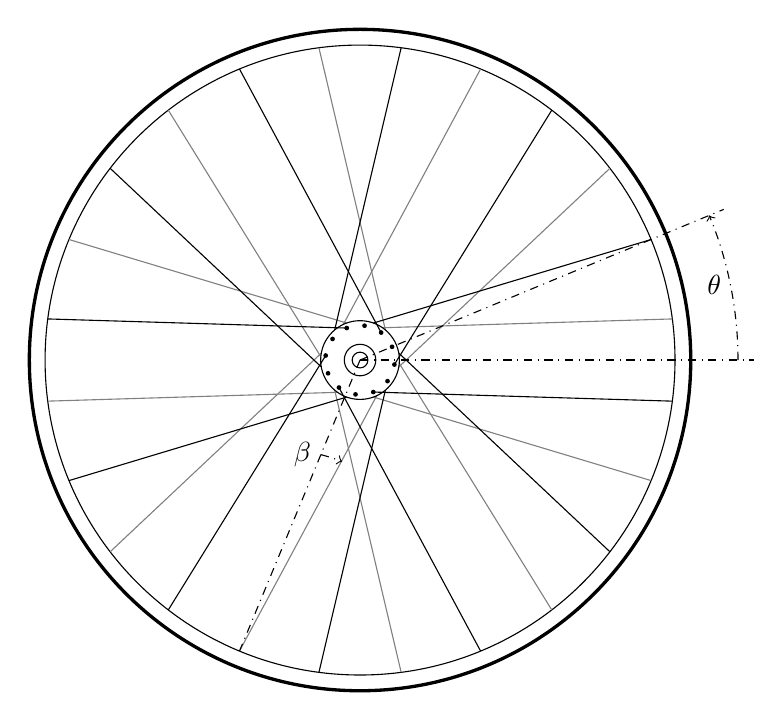
\begin{tikzpicture}
% Wheel components
%-----------------------------------------------------------%
% rim ID
  \draw (0,0)  circle[radius = 4 cm];
% rim OD
  \draw[very thick] circle[radius = 4.2 cm];
% Trailing DS spokes 
        \foreach \x in {7.5,67.5,...,307.5}
        { \draw[gray] (\x:0.44cm) -- (\x - 60:4cm);}
% leading DS spokes
    \foreach \x in {37.5,97.5,...,337.5}
        { \draw[gray] (\x:0.44cm) -- (\x + 60:4cm);}
% Interior NDS spokes
    \foreach \x in {22.5,82.5,...,322.5}
      {\draw (\x:0.44cm) -- (\x - 60:4cm);}
% cover over spoke ends
    \fill [color=white] circle[radius=0.5];
%hub flange
    \draw circle[radius = 0.5 cm];
% axle OD
    \draw circle[radius = 0.1 cm];
% bearing OD
    \draw circle [radius=0.2cm];
% Exterior NDS spokes and spoke holes
\foreach \x in {52.5,112.5,...,352.5} 
        { \fill (\x:0.44 cm)  circle [radius =0.03 cm];
        \draw (\x:0.44cm) -- (\x + 60:4cm);}
% Interior NDS spoke holes
    \foreach \x in {22.5,82.5,...,322.5}
      { \fill (\x:0.44 cm)  circle [radius =0.03 cm];}
%-----------------------------------------------------------%
% rim angle theta
\draw[dash dot]  (0,0) --(5 cm, 0);
\draw[dash dot] (0,0) -- (22.5:5 cm);
\draw[dash dot,->] (4.8 cm,0) arc [start angle =0, end angle = 22.5, radius = 4.8 cm] ;
\draw (12:4.6cm) node{$\theta$};
% beta spoke angle
\draw[dash dot] (0,0) -- (247.5:4cm);
\draw[dash dot,->] (247.5:1.3cm) node[left]{$\beta$} arc [start angle =75, end angle = 69, radius = 2.7 cm] ;

\end{tikzpicture}
\end{document}